% TikZ Gallery: twelve vector diagrams for mathematics, physics, chemistry and computer science.
\documentclass[11pt,a4paper]{article}

\usepackage[T1]{fontenc}
\usepackage[utf8]{inputenc}
\usepackage[a4paper,top=2.5cm,bottom=2.3cm,left=2.2cm,right=2.2cm]{geometry}
\usepackage{libertinus}
\usepackage{microtype}
\usepackage{amsmath,amssymb}
\usepackage{float}
\usepackage[font=small,labelfont=bf,format=hang]{caption}
\usepackage{subcaption}
\usepackage{siunitx}
\usepackage{tikz}
\usetikzlibrary{arrows.meta,calc,positioning,shapes.geometric,shapes.misc,automata,mindmap,trees}
\usepackage{tikz-cd}
\usepackage{pgfplots}
\pgfplotsset{compat=1.18}
\usepackage[siunitx]{circuitikz}
\usepackage{chemfig}
\usepackage{fancyhdr}
\usepackage[colorlinks=true,linkcolor=blue!50!black,urlcolor=blue!50!black]{hyperref}

\setchemfig{atom sep=2.2em,bond offset=2pt}
\pagestyle{fancy}
\fancyhf{}
\fancyhead[L]{\small\textsc{TikZ Gallery}}
\fancyhead[R]{\small N'sol\'e Samson Yamontche}
\fancyfoot[C]{\small\thepage}
\renewcommand{\headrulewidth}{0.3pt}
\setlength{\headheight}{14pt}
\newcommand{\libs}[1]{\emph{Libraries:} #1.}

\begin{document}

% ------------------------------------------------------------------ cover
\begin{titlepage}
  \centering
  \vspace*{2.6cm}
  {\fontsize{40}{44}\selectfont\bfseries TikZ Gallery\par}
  \vspace{0.5cm}
  {\Large Vector diagrams for mathematics, physics,\\ chemistry and computer science\par}
  \vspace{1.6cm}
  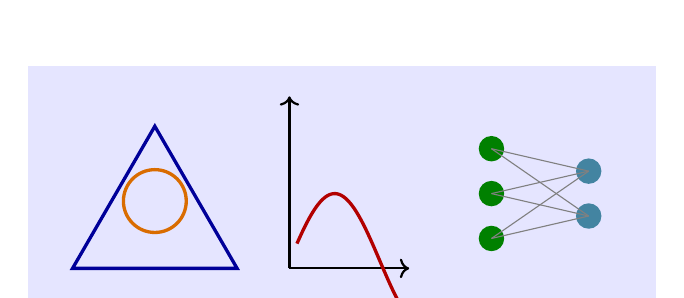
\begin{tikzpicture}[scale=0.95]
    \fill[blue!10] (-4.2,-1.5) rectangle (4.2,1.7);
    \draw[blue!60!black,very thick] (-3.6,-1) -- (-1.4,-1) -- (-2.5,0.9) -- cycle;
    \draw[orange!85!black,very thick] (-2.5,-0.1) circle (0.42);
    \draw[->,thick] (-0.7,-1) -- (-0.7,1.3);
    \draw[->,thick] (-0.7,-1) -- (0.9,-1);
    \draw[red!70!black,very thick,domain=-0.6:0.8,samples=60] plot (\x,{-0.9+0.9*sin(deg(2.6*(\x+0.7)))});
    \foreach \i in {0,1,2}{\fill[green!50!black] (2.0,{0.6-0.6*\i}) circle (0.17);}
    \foreach \i in {0,1}{\fill[cyan!60!black] (3.3,{0.3-0.6*\i}) circle (0.17);}
    \foreach \i in {0,1,2}{\foreach \j in {0,1}{\draw[gray] (2.0,{0.6-0.6*\i})--(3.3,{0.3-0.6*\j});}}
  \end{tikzpicture}
  \vfill
  {\large N'sol\'e Samson Yamontche\par}
  \vspace{2pt}
  {\small\url{https://samsonyamontchensolegit.github.io}\par}
  \vspace{1.2cm}
\end{titlepage}

\setcounter{page}{2}
\section*{Contents}
\listoffigures
\bigskip
\noindent
Every figure in this document is drawn directly in \LaTeX{} with TikZ and its libraries:
no external images, no raster graphics. The drawings scale without loss of quality and use the same fonts as the text.
\clearpage

% ------------------------------------------------------------------ 1 neural network
\begin{figure}[H]
  \centering
  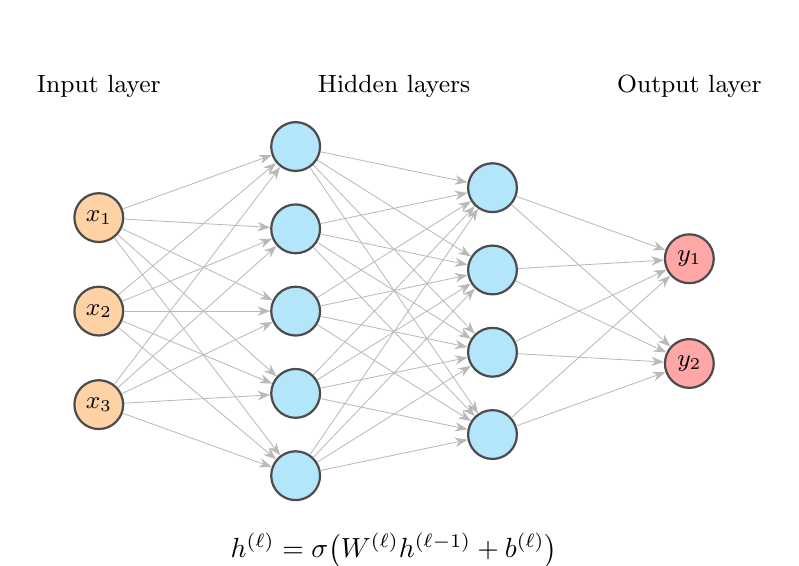
\begin{tikzpicture}[x=2.5cm,y=0.95cm,
      neuron/.style={circle,draw=black!70,thick,minimum size=0.62cm,inner sep=0pt},
      nin/.style={neuron,fill=orange!35}, nhid/.style={neuron,fill=cyan!30}, nout/.style={neuron,fill=red!35},
      conn/.style={gray!55,-{Stealth[length=1.6mm]},line width=0.3pt}]
    \foreach \i in {1,...,3}{\node[nin] (I\i) at (0,{(2-\i)*1.25}) {\small$x_{\i}$};}
    \foreach \i in {1,...,5}{\node[nhid] (H\i) at (1,{(3-\i)*1.1}) {};}
    \foreach \i in {1,...,4}{\node[nhid] (K\i) at (2,{(2.5-\i)*1.1}) {};}
    \foreach \i in {1,...,2}{\node[nout] (O\i) at (3,{(1.5-\i)*1.4}) {\small$y_{\i}$};}
    \foreach \i in {1,...,3}{\foreach \j in {1,...,5}{\draw[conn] (I\i)--(H\j);}}
    \foreach \i in {1,...,5}{\foreach \j in {1,...,4}{\draw[conn] (H\i)--(K\j);}}
    \foreach \i in {1,...,4}{\foreach \j in {1,...,2}{\draw[conn] (K\i)--(O\j);}}
    \node at (0,3.0) {\small Input layer};
    \node at (1.5,3.0) {\small Hidden layers};
    \node at (3,3.0) {\small Output layer};
    \node at (1.5,-3.2) {$h^{(\ell)}=\sigma\!\left(W^{(\ell)}h^{(\ell-1)}+b^{(\ell)}\right)$};
  \end{tikzpicture}
  \caption[A feed-forward neural network]{A feed-forward neural network with two hidden layers. \libs{arrows.meta}}
\end{figure}

% ------------------------------------------------------------------ 2 commutative diagrams
\begin{figure}[H]
  \centering
  \begin{tikzcd}[row sep=2.4em,column sep=3.4em]
    G \arrow[r,"\varphi"] \arrow[d,"\pi"'] & H \\
    G/\ker\varphi \arrow[ur,dashed,"\bar\varphi"'] &
  \end{tikzcd}
  \qquad\qquad
  \begin{tikzcd}[row sep=2.4em,column sep=2.4em]
    0 \arrow[r] & A \arrow[r,"f"] \arrow[d,"\alpha"'] & B \arrow[r,"g"] \arrow[d,"\beta"'] & C \arrow[r] \arrow[d,"\gamma"'] & 0 \\
    0 \arrow[r] & A' \arrow[r,"f'"'] & B' \arrow[r,"g'"'] & C' \arrow[r] & 0
  \end{tikzcd}
  \caption[Commutative diagrams]{Commutative diagrams: the first isomorphism theorem (left) and a morphism of short exact sequences (right). \libs{tikz-cd}}
\end{figure}
\clearpage

% ------------------------------------------------------------------ 3 flowchart
\begin{figure}[H]
  \centering
  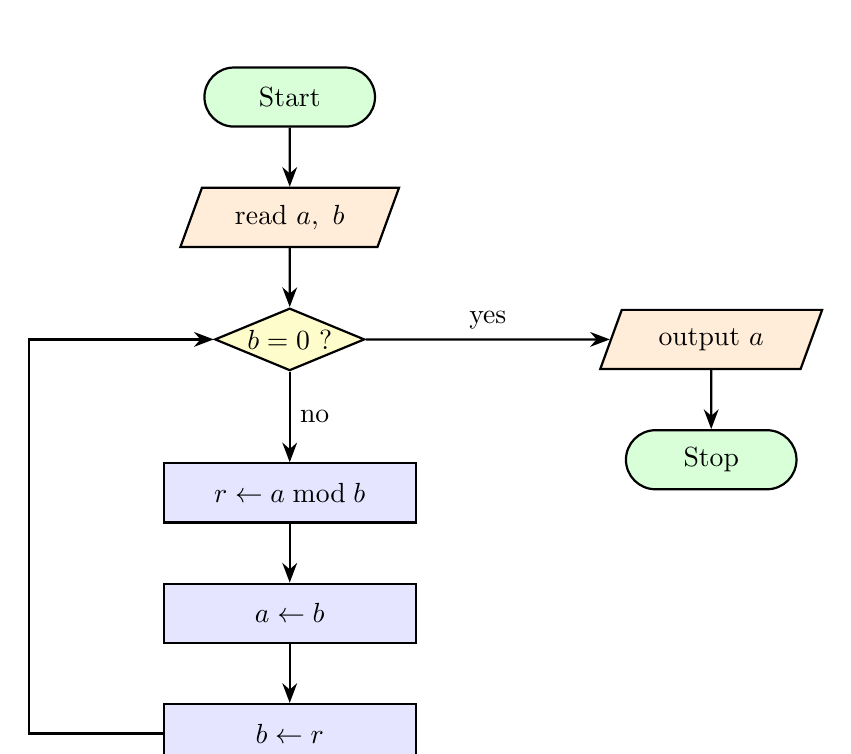
\begin{tikzpicture}[node distance=0.75cm,
      term/.style={rounded rectangle,draw,thick,fill=green!15,minimum width=2.4cm,minimum height=0.75cm},
      proc/.style={rectangle,draw,thick,fill=blue!10,minimum width=3.2cm,minimum height=0.75cm},
      io/.style={trapezium,trapezium left angle=70,trapezium right angle=110,draw,thick,fill=orange!15,minimum height=0.75cm},
      dec/.style={diamond,aspect=2.4,draw,thick,fill=yellow!20,inner sep=1pt},
      arr/.style={-{Stealth[length=2.5mm]},thick}]
    \node[term] (start) {Start};
    \node[io,below=of start] (read) {read $a,\ b$};
    \node[dec,below=of read] (test) {$b=0$ ?};
    \node[proc,below=1.15cm of test] (r) {$r\leftarrow a \bmod b$};
    \node[proc,below=of r] (a) {$a\leftarrow b$};
    \node[proc,below=of a] (b) {$b\leftarrow r$};
    \node[io,right=3.1cm of test] (res) {output $a$};
    \node[term,below=of res] (stop) {Stop};
    \draw[arr] (start)--(read);
    \draw[arr] (read)--(test);
    \draw[arr] (test)--node[right]{no}(r);
    \draw[arr] (r)--(a);
    \draw[arr] (a)--(b);
    \draw[arr] (b.west)--++(-1.7,0)|-(test.west);
    \draw[arr] (test)--node[above]{yes}(res);
    \draw[arr] (res)--(stop);
  \end{tikzpicture}
  \caption[Flowchart of Euclid's algorithm]{Flowchart of Euclid's algorithm for the greatest common divisor. \libs{shapes.geometric, positioning}}
\end{figure}

% ------------------------------------------------------------------ 4 automata
\begin{figure}[H]
  \centering
  \begin{subfigure}[b]{0.47\linewidth}
    \centering
    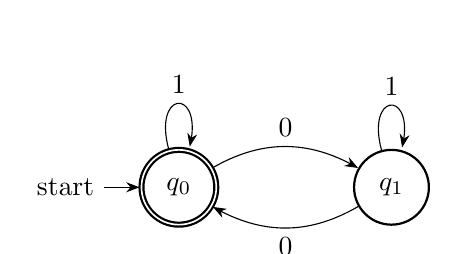
\begin{tikzpicture}[->,>=Stealth,auto,node distance=2.7cm,every state/.style={thick,minimum size=0.95cm}]
      \node[state,initial,accepting] (q0) {$q_0$};
      \node[state,right of=q0] (q1) {$q_1$};
      \path (q0) edge[bend left] node {0} (q1)
                 edge[loop above] node {1} ()
            (q1) edge[bend left] node {0} (q0)
                 edge[loop above] node {1} ();
    \end{tikzpicture}
    \caption{Even number of $0$s.}
  \end{subfigure}\hfill
  \begin{subfigure}[b]{0.50\linewidth}
    \centering
    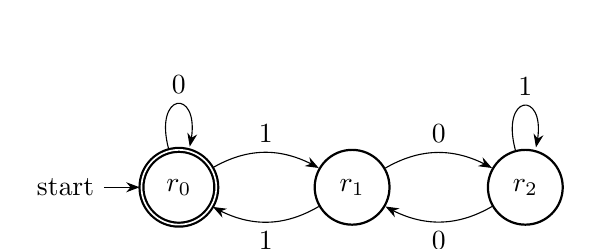
\begin{tikzpicture}[->,>=Stealth,auto,node distance=2.2cm,every state/.style={thick,minimum size=0.95cm}]
      \node[state,initial,accepting] (r0) {$r_0$};
      \node[state,right of=r0] (r1) {$r_1$};
      \node[state,right of=r1] (r2) {$r_2$};
      \path (r0) edge[loop above] node {0} ()
                 edge[bend left] node {1} (r1)
            (r1) edge[bend left] node {1} (r0)
                 edge[bend left] node {0} (r2)
            (r2) edge[bend left] node {0} (r1)
                 edge[loop above] node {1} ();
    \end{tikzpicture}
    \caption{Binary numbers divisible by $3$.}
  \end{subfigure}
  \caption[Finite automata]{Two deterministic finite automata. \libs{automata}}
\end{figure}
\clearpage

% ------------------------------------------------------------------ 5 geometry
\begin{figure}[H]
  \centering
  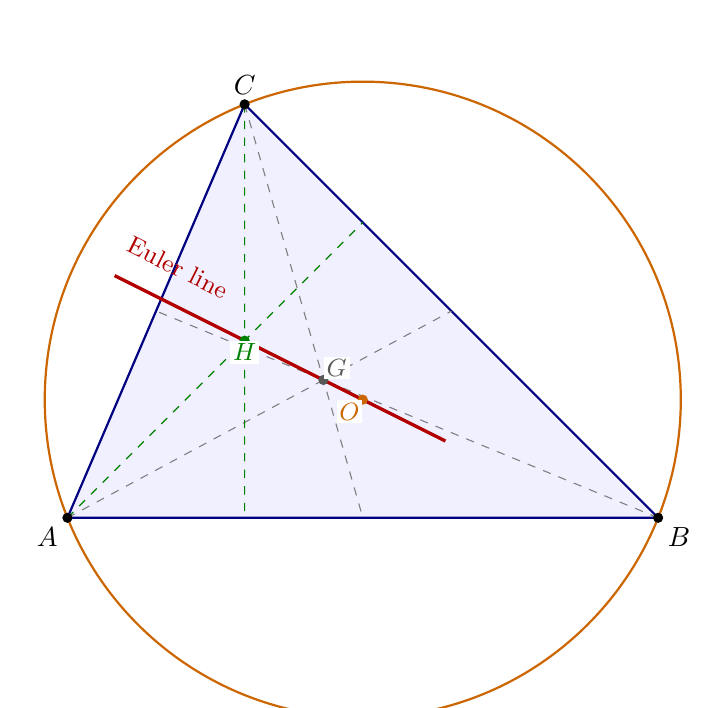
\begin{tikzpicture}[scale=1.25,>=Stealth,dot/.style={circle,fill,inner sep=1.3pt}]
    \coordinate (A) at (0,0);
    \coordinate (B) at (6,0);
    \coordinate (C) at (1.8,4.2);
    \coordinate (O) at (3,1.2);
    \coordinate (G) at (2.6,1.4);
    \coordinate (H) at (1.8,1.8);
    \coordinate (Ma) at ($(B)!0.5!(C)$);
    \coordinate (Mb) at ($(A)!0.5!(C)$);
    \coordinate (Mc) at ($(A)!0.5!(B)$);
    \draw[orange!80!black,thick] (O) circle [radius=3.2311];
    \draw[blue!50!black,thick,fill=blue!6] (A)--(B)--(C)--cycle;
    \draw[gray,dashed] (A)--(Ma) (B)--(Mb) (C)--(Mc);
    \draw[green!50!black,dashed] (C)--(1.8,0) (A)--(3,3);
    \draw[red!70!black,very thick] ($(O)!-0.7!(H)$) -- ($(O)!2.1!(H)$);
    \node[dot] at (A) {}; \node[dot] at (B) {}; \node[dot] at (C) {};
    \node[dot,fill=orange!80!black] at (O) {};
    \node[dot,fill=gray!70!black] at (G) {};
    \node[dot,fill=green!50!black] at (H) {};
    \node[below left] at (A) {$A$}; \node[below right] at (B) {$B$}; \node[above] at (C) {$C$};
    \node[font=\small,below left,orange!80!black,fill=white,inner sep=1pt] at (O) {$O$};
    \node[font=\small,above right,gray!70!black,fill=white,inner sep=1pt] at (G) {$G$};
    \node[font=\small,below,green!50!black,fill=white,inner sep=1pt] at (H) {$H$};
    \node[red!70!black,font=\small,rotate=-26.6,above,yshift=7pt] at (0.95,2.2) {Euler line};
  \end{tikzpicture}
  \caption[Euler line of a triangle]{A triangle with its circumcircle, medians and altitudes. The circumcentre $O$, the centroid $G$ and the orthocentre $H$ lie on the Euler line, with $OG:GH=1:2$. \libs{calc}}
\end{figure}

% ------------------------------------------------------------------ 6 unit circle
\begin{figure}[H]
  \centering
  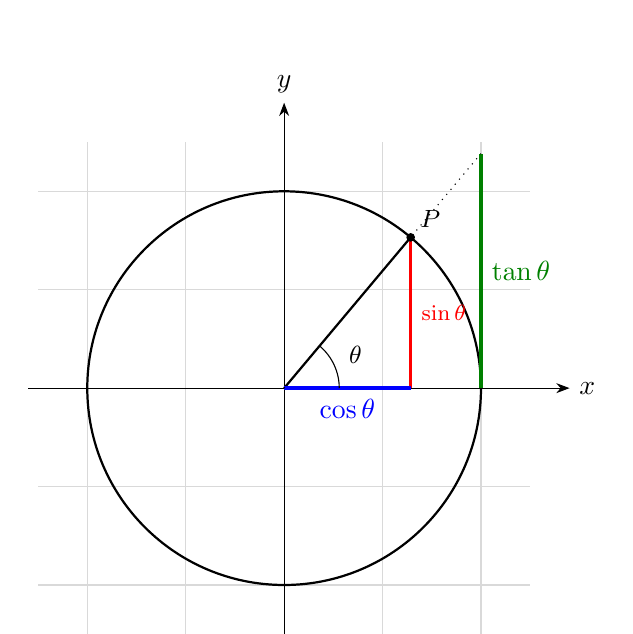
\begin{tikzpicture}[scale=2.5,>=Stealth]
    \def\a{50}
    \draw[gray!30,step=0.5] (-1.25,-1.25) grid (1.25,1.25);
    \draw[->] (-1.3,0)--(1.45,0) node[right]{$x$};
    \draw[->] (0,-1.3)--(0,1.45) node[above]{$y$};
    \draw[thick] (0,0) circle (1);
    \draw[thick] (0,0)--({cos(\a)},{sin(\a)});
    \draw[red,very thick] ({cos(\a)},0)--({cos(\a)},{sin(\a)}) node[midway,right,font=\footnotesize]{$\sin\theta$};
    \draw[blue,very thick] (0,0)--({cos(\a)},0) node[midway,below]{$\cos\theta$};
    \draw[green!50!black,very thick] (1,0)--(1,{tan(\a)}) node[midway,right]{$\tan\theta$};
    \draw[dotted] (0,0)--(1,{tan(\a)});
    \draw (0.28,0) arc (0:\a:0.28);
    \node at ({0.4*cos(\a/2)},{0.4*sin(\a/2)}) {\small$\theta$};
    \fill ({cos(\a)},{sin(\a)}) circle (0.022);
    \node[above right,font=\small] at ({cos(\a)},{sin(\a)}) {$P$};
  \end{tikzpicture}
  \caption[The unit circle]{The unit circle with the three basic trigonometric functions of the angle $\theta=50^{\circ}$, with $P=(\cos\theta,\sin\theta)$. \libs{standard TikZ}}
\end{figure}
\clearpage

% ------------------------------------------------------------------ 7 pgfplots
\begin{figure}[H]
  \centering
  \begin{subfigure}[b]{0.48\linewidth}
    \centering
    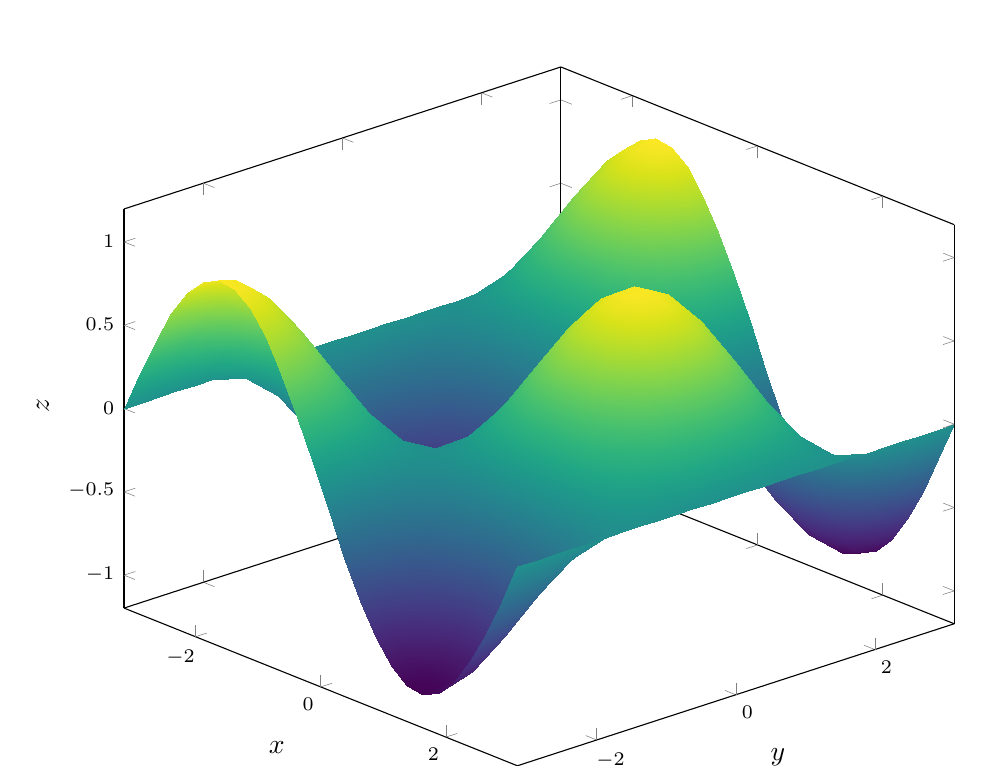
\begin{tikzpicture}
      \begin{axis}[width=\linewidth,view={48}{28},xlabel=$x$,ylabel=$y$,zlabel=$z$,colormap/viridis,
          domain=-3.1416:3.1416,y domain=-3.1416:3.1416,samples=26,tick label style={font=\scriptsize}]
        \addplot3[surf,shader=interp] {sin(deg(x))*cos(deg(y))};
      \end{axis}
    \end{tikzpicture}
    \caption{The surface $z=\sin x\cos y$.}
  \end{subfigure}\hfill
  \begin{subfigure}[b]{0.48\linewidth}
    \centering
    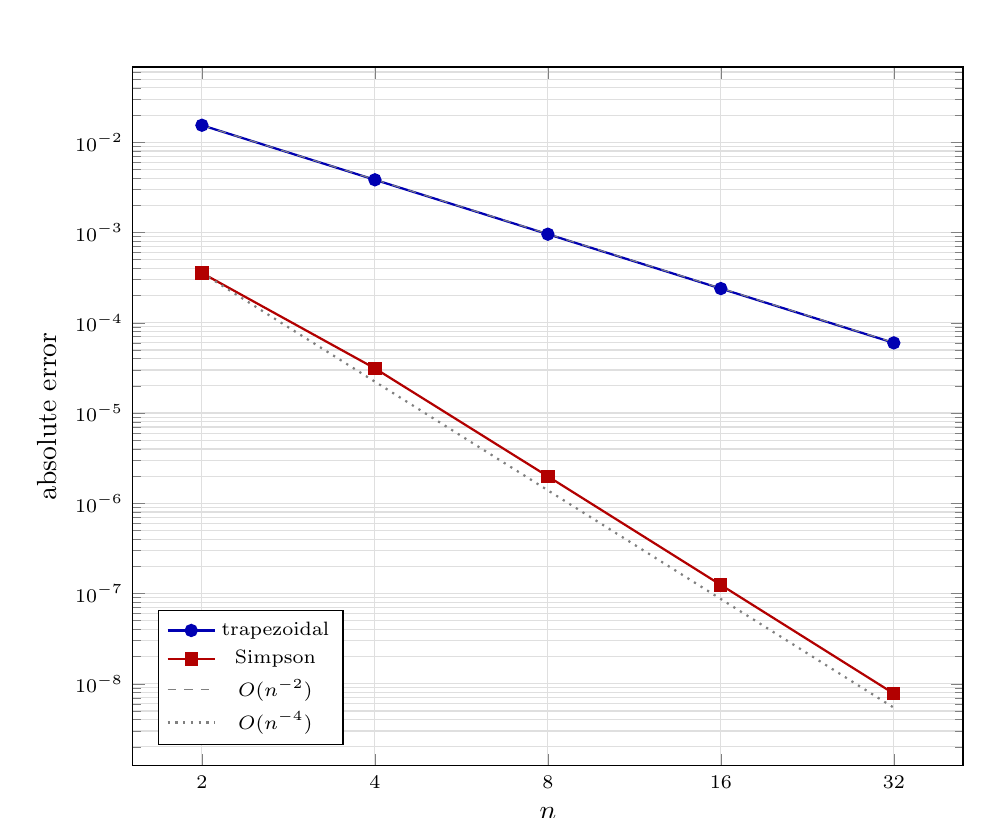
\begin{tikzpicture}
      \begin{axis}[width=\linewidth,xmode=log,ymode=log,log basis x=2,
          xtick={2,4,8,16,32},xticklabels={2,4,8,16,32},xlabel={$n$},ylabel={absolute error},
          grid=both,grid style={gray!25},legend pos=south west,legend style={font=\scriptsize},
          tick label style={font=\scriptsize}]
        \addplot[blue!70!black,mark=*,thick] coordinates {(2,1.545e-2) (4,3.840e-3) (8,9.585e-4) (16,2.395e-4) (32,5.988e-5)};
        \addlegendentry{trapezoidal}
        \addplot[red!70!black,mark=square*,thick] coordinates {(2,3.563e-4) (4,3.125e-5) (8,1.988e-6) (16,1.246e-7) (32,7.795e-9)};
        \addlegendentry{Simpson}
        \addplot[gray,dashed,domain=2:32] {1.545e-2*(2/x)^2};
        \addlegendentry{$O(n^{-2})$}
        \addplot[gray,dotted,thick,domain=2:32] {3.563e-4*(2/x)^4};
        \addlegendentry{$O(n^{-4})$}
      \end{axis}
    \end{tikzpicture}
    \caption{Errors for $\int_0^1 e^{-x^2}\,\mathrm{d}x$.}
  \end{subfigure}
  \caption[Surface and convergence plots]{Plots with \texttt{pgfplots}: a 3D surface (left) and a log--log convergence study with the reference slopes (right). \libs{pgfplots}}
\end{figure}

% ------------------------------------------------------------------ 8 circuit
\begin{figure}[H]
  \centering
  \begin{circuitikz}[american]
    \draw (0,0) to[sV,l=$v_s(t)$] (0,3)
          to[R=$R$,i>=$i(t)$] (3,3)
          to[L=$L$] (6,3)
          to[C=$C$] (6,0) -- (0,0);
    \node at (3,1.3) {$v_s=R\,i+L\,\dfrac{\mathrm{d}i}{\mathrm{d}t}+\dfrac1C\displaystyle\int i\,\mathrm{d}t$};
  \end{circuitikz}
  \caption[Series RLC circuit]{A series RLC circuit driven by a sinusoidal voltage source. \libs{circuitikz}}
\end{figure}
\clearpage

% ------------------------------------------------------------------ 9 chemistry
\begin{figure}[H]
  \centering
  \schemestart
    \chemfig{H_3C-C(=[:60]O)-OH}
    \+
    \chemfig{HO-CH_2-CH_3}
    \arrow{<=>[$\mathrm{H^{+}}$]}
    \chemfig{H_3C-C(=[:60]O)-O-CH_2-CH_3}
    \+
    \chemfig{H_2O}
  \schemestop

  \vspace{1.4cm}
  \begin{tabular}{@{}ccc@{}}
    \chemfig{*6(=-=-=-)} \hspace{1.6cm} & \chemfig{*6((-OH)=-=-=-)} \hspace{1.6cm} & \chemfig{*6((-CH_3)=-=-=-)}\\[3pt]
    \small benzene & \small phenol & \small toluene
  \end{tabular}
  \caption[Chemical structures]{Fischer esterification of acetic acid with ethanol, and three aromatic compounds. \libs{chemfig}}
\end{figure}

% ------------------------------------------------------------------ 10 venn
\begin{figure}[H]
  \centering
  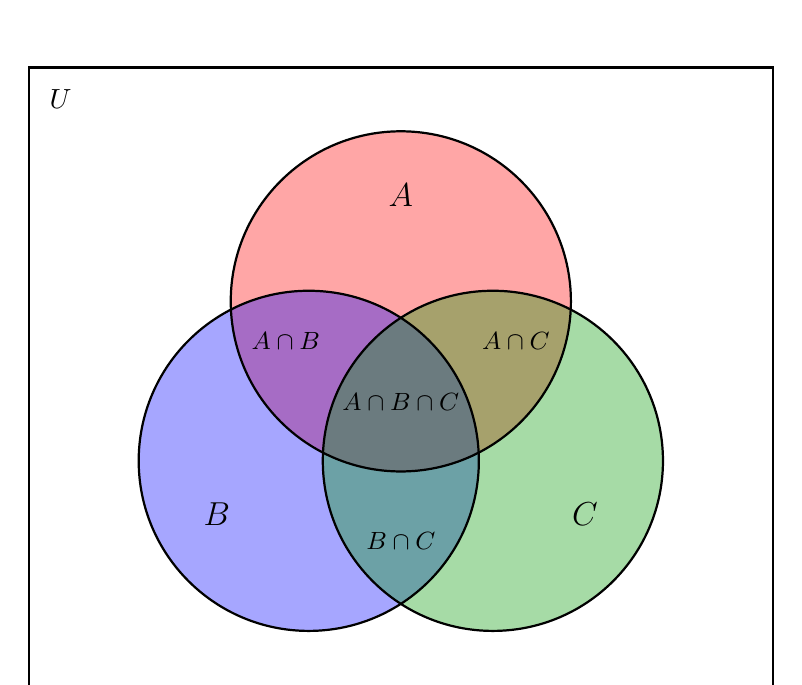
\begin{tikzpicture}[scale=1.35]
    \draw[thick] (-3.5,-2.7) rectangle (3.5,3.2);
    \node at (-3.2,2.9) {$U$};
    \begin{scope}[fill opacity=0.35]
      \fill[red]   (90:1)  circle (1.6);
      \fill[blue]  (210:1) circle (1.6);
      \fill[green!60!black] (330:1) circle (1.6);
    \end{scope}
    \draw[thick] (90:1) circle (1.6);
    \draw[thick] (210:1) circle (1.6);
    \draw[thick] (330:1) circle (1.6);
    \node[font=\large] at (90:2.0) {$A$};
    \node[font=\large] at (210:2.0) {$B$};
    \node[font=\large] at (330:2.0) {$C$};
    \node[font=\small] at (150:1.25) {$A\cap B$};
    \node[font=\small] at (30:1.25) {$A\cap C$};
    \node[font=\small] at (270:1.25) {$B\cap C$};
    \node[font=\small] at (0,0.05) {$A\cap B\cap C$};
  \end{tikzpicture}
  \caption[Venn diagram]{A Venn diagram of three sets inside a universe $U$. \libs{standard TikZ}}
\end{figure}
\clearpage

% ------------------------------------------------------------------ 11 mindmap
\begin{figure}[H]
  \centering
  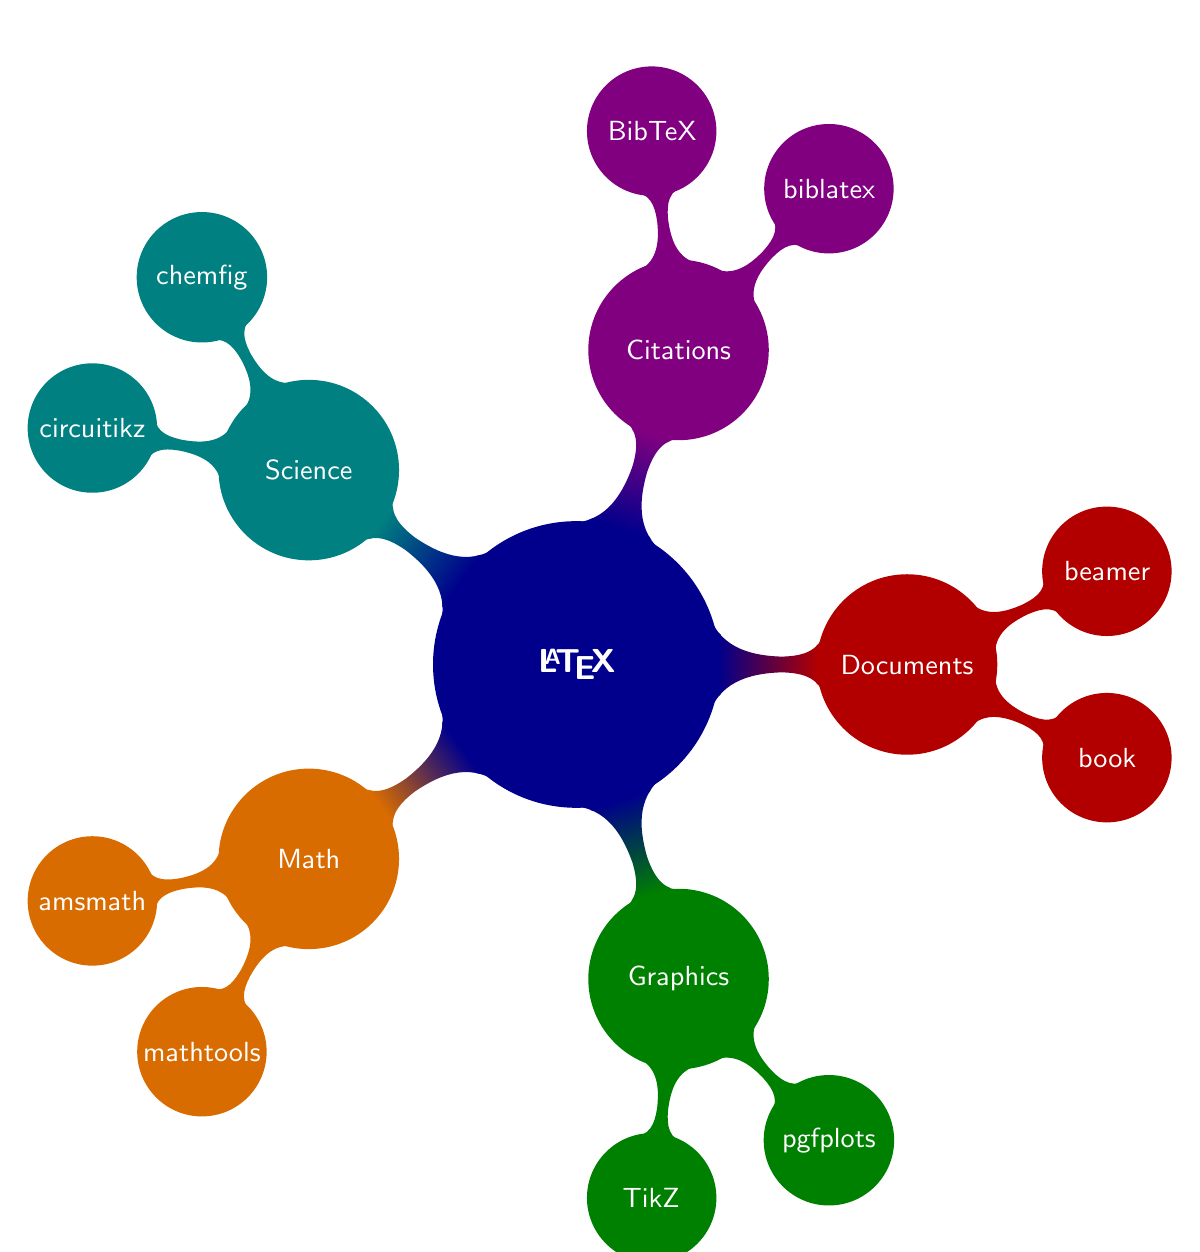
\begin{tikzpicture}[mindmap,grow cyclic,
      every node/.style={concept,text=white,font=\sffamily},
      concept color=blue!55!black,
      root concept/.append style={font=\large\bfseries\sffamily,minimum size=2.4cm},
      level 1 concept/.append style={level distance=4.2cm,sibling angle=72,font=\small\bfseries\sffamily},
      level 2 concept/.append style={level distance=2.8cm,sibling angle=50,font=\scriptsize\sffamily,minimum size=0.95cm}]
    \node[root concept] {\LaTeX}
      child[concept color=orange!85!black] {node[concept] {Math} child {node[concept] {amsmath}} child {node[concept] {mathtools}}}
      child[concept color=green!50!black]  {node[concept] {Graphics} child {node[concept] {TikZ}} child {node[concept] {pgfplots}}}
      child[concept color=red!70!black]    {node[concept] {Documents} child {node[concept] {book}} child {node[concept] {beamer}}}
      child[concept color=violet]          {node[concept] {Citations} child {node[concept] {biblatex}} child {node[concept] {BibTeX}}}
      child[concept color=teal]            {node[concept] {Science} child {node[concept] {chemfig}} child {node[concept] {circuitikz}}};
  \end{tikzpicture}
  \caption[A mind map of the \LaTeX{} ecosystem]{A mind map of the \LaTeX{} ecosystem. \libs{mindmap, trees}}
\end{figure}

% ------------------------------------------------------------------ 12 physics
\begin{figure}[H]
  \centering
  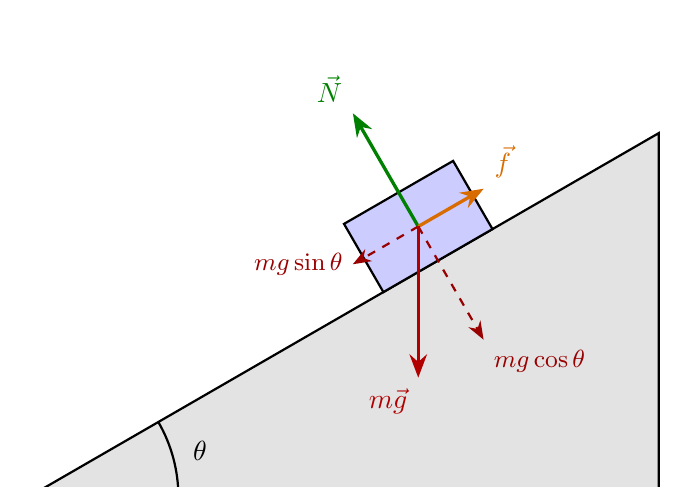
\begin{tikzpicture}[>=Stealth]
    \def\th{30}
    \fill[gray!22] (0,0)--(8,0)--(8,{8*tan(\th)})--cycle;
    \draw[thick] (0,0)--(8,0)--(8,{8*tan(\th)})--cycle;
    \begin{scope}[rotate=\th]
      \draw[thick,fill=blue!20] (5.2,0) rectangle (6.8,1.0);
      \coordinate (C) at (6.0,0.5);
      \draw[->,very thick,green!50!black] (C)--++(0,1.66) node[above left]{$\vec N$};
      \draw[->,very thick,orange!85!black] (C)--++(0.96,0) node[above right]{$\vec f$};
      \draw[->,dashed,thick,red!60!black] (C)--++(-0.96,0) node[left,font=\small]{$mg\sin\theta$};
      \draw[->,dashed,thick,red!60!black] (C)--++(0,-1.66) node[below right,font=\small]{$mg\cos\theta$};
    \end{scope}
    \draw[->,very thick,red!70!black] (C)--++(0,-1.92) node[below left]{$m\vec g$};
    \draw[thick] (1.9,0) arc[start angle=0,end angle=\th,radius=1.9];
    \node at ({2.25*cos(\th/2)},{2.25*sin(\th/2)}) {$\theta$};
  \end{tikzpicture}
  \caption[Block on an inclined plane]{Free-body diagram of a block at rest on an inclined plane: $N=mg\cos\theta$ and $f=mg\sin\theta$. \libs{standard TikZ}}
\end{figure}

\end{document}





